
\documentclass[a4paper]{article}

\usepackage{graphicx}
\usepackage{listings}
\usepackage{indentfirst}
\usepackage{float}
%\usepackage[T1]{fontenc}                % F�r svenska bokst�ver
%\usepackage[swedish]{babel}             % F�r svensk avstavning och svenska
                                        % rubriker (t ex "inneh�llsf�rteckning)
\title{Programming Project, Database Technology}
\author{Tim Dolck dat11tdo@student.lu.se \\ 
Julian Kron� dat11jkr@student.lu.se \\
Christopher Nilsson dat11cni@student.lu.se}
%\date{}           % Blir dagens datum om det utel�mnas

\begin{document}
\lstset{language=SQL}

\maketitle
\newpage
\section{Introduction}

This is our project for the course Database Technology at LTH.
The assignment brought to us was to build a program for a cookie factory for a 
fictional customer, Krusty Cookies.
They needed a program to help them manage their production, deliveries and 
orders. The implementation of such a system therefore needs to contain a 
database-system and straight forward user interface for Krusty Cookies.

Our implementation is a pilot program for demonstration purposes and
laying the ground work for further development. In this pilot version
it is possible to create, search and block pallets.
Throughout the project we faced different challenges setting up a local-
server, planning effective database relations, managing the database and 
designing a user-friendly interface. To implement the system we used the
programming language Scala and the Play-framework.

\section{Requirements}

Krusty Cookies database system is built with the simplest possible interface 
to make sure all employees are able to use it. At this point the system is 
only a test system with all aspects of production implemented although the 
database is prepared for future development!

\subsection{Production}
\textit{A pallet is considered to be produced when the pallet label is read at 
the entrance to the deepfreeze storage. The pallet number, product name, and 
date and time of production is registered in the database. The pallet number 
is unique. At any time, we must be able to check how many pallets of a product 
that have been produced during a specific time.}

In our system we don't have access to a barcode scanner, therefor a pallet is
created on button clicks in the user-interface.

\subsection{Raw Materials}
\textit{When a pallet is produced, the raw materials storage must be updated. 
We must be able to check the amount in store of each ingredient, and to see 
when, and how much of, an ingredient was last delivered into storage.}

When a pallet is produced in our system the raw materials storage database is 
updated accordingly. The rest was not part of our implementation because it 
was stated so in the assignment description. Although the database supports 
all of the stated data.

\subsection{Recipes}
\textit{We need an interface to the collection of recipes (appendix A), where 
we can study and update recipes. We also need a facility for entering new 
recipes. We don�t change recipes during production.}

This is not implemented because it was not included in the assignment. The 
database contains recipes which is used to update the available raw materials 
when a pallet is created.

\subsection{Produced Pallets}
\textit{As we mentioned earlier, pallets in the deep-freeze storage may be 
blocked. An order to block a pallet will always come before the pallet has 
been delivered. This is due to the new investments in our laboratory, where 
the analysis process is completely automated. We must be able to trace each 
pallet. For instance, we need to see all information about a pallet with a 
given number (the contents of the pallet, the location of the pallet, if the 
pallet is delivered and in that case to whom, etc.). We must also be able to 
see which pallets that contain a certain product and which pallets that have 
been produced during a certain time interval. Blocked products are of special 
interest. We need to find out which products that are blocked, and also which 
pallets that contain a certain blocked product. Finally, we must be able to 
check which pallets that have been delivered to a given customer, and the date 
and time of delivery.}

Our system supports blocking of pallets. Everything regarding delivery and 
tracing of pallets is to be implemented in a future version. Although it is
very simple to search and filter the produced pallets before delivery.

\subsection{Orders and Production Planning}
\textit{Orders must be registered in the database. For production planning 
purposes, we must have a facility to see all orders that are to be delivered 
during a specific time period. The production planning is manual. At the end 
of each week, production for the following week is planned, using the orders 
for the following weeks as input. We cannot produce �on demand�, since it 
takes time to set up a production line for a new kind of cookie (mixers have to
be cleaned, for example).}

Nothing regarding orders are implemented in the user interface in this version.
The database although supports it. 

\subsection{Delivery}
\textit{Before pallets are loaded into the freezer trucks, a loading order is 
created. The order contains information regarding the customers and the number 
of pallets to be delivered. When pallets are taken out of deep-freeze storage 
the pallet label is read. When the truck is loaded, the driver receives a 
loading bill (identical to the loading order, but contains a field where the 
customer can acknowledge reception of the delivery). The loading bill data 
need not be saved in the database. When the loading bill has been printed, the 
data regarding delivered pallets must be updated with customer data and date 
of delivery.}

Nothing about delivery is implemented in this version of the system.

\section{Outline}
Our product is built in play framework. It is a web application framework with support for programming in scala. Play also enables us to easy use a model-view-controller modell, which we have. The view section is mostly built up by html-templates. These templates are filled up with data from scala-variables. The model \& controller section are both written in scala. 

The product uses jdbc as databasemanager. The controller section of the program has the connection with the database. It handles all the SQL-queries and sends them to the database. For every method the controller sets up a connection with the database, sends the queries, gets the result and closes the connection.

\section{Model}

\subsection{E/R Diagram}

An overview of the database design can be seen in figure~\ref{model}.

\begin{figure}[H]
  \centering
  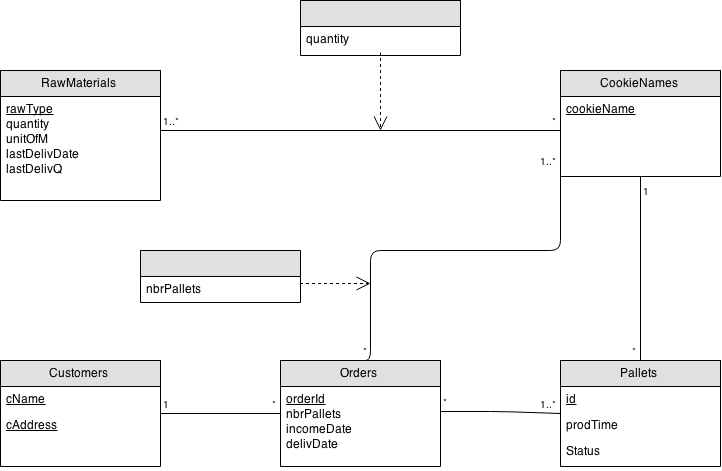
\includegraphics[width=\textwidth]{cookies.png}
  \caption{An UML diagram illustrating the database design.}
  \label{model}
\end{figure}

\subsection{Relations}

The relations extracted from the database design are as follows:

\noindent
RawMaterials(\underline{rawType}, quantity, unitOfM, lastDelivDate, lastDelivQ) \\
CookieNames(\underline{cookieName}) \\
RecipeDetails(\underline{\emph{rawType, cookieName}}, quantity) \\
Pallets(\underline{id}, prodTime, Status, \emph{cookieName, orderId}) \\
Customers(\underline{cName, cAddress}) \\
Orders(\underline{orderId}, nbrPallets, incomeDate, delivDate, \emph{cName, cAddress}) \\
OrderDetails(\underline{\emph{orderId, cookieName}}, nbrPallets)
\indent

There are no other functional dependencies except for the key dependencies, so the relations are in
BCNF.

\section{Statements}

The statements used when creating the database:

\begin{lstlisting}[frame=single]
--
-- Disable foreign key checks temporarily so 
-- tables can be deleted in arbitrary order, 
-- and so that insertion is faster.

set FOREIGN_KEY_CHECKS = 0;

-- Drop the tables if they already exist.

drop table if exists RawMaterials;
drop table if exists RecipeDetails;
drop table if exists CookieNames;
drop table if exists Pallets;
drop table if exists OrderDetails;
drop table if exists Orders;
drop table if exists Customers;

-- Create the tables.

create table RawMaterials (
    rawType     varchar(30) not null,
    quantity    integer default 100000000 
      check (quantity >= 0),
    unitOfM     enum('g', 'ml') not null,
    lastDeliv   datetime,
    lastDelivQ  integer,
    primary key (rawType)
);

create table RecipeDetails (
    cookieName  varchar(20) not null,
    rawType     varchar(30) not null,
    quantity    integer not null,
    primary key (cookieName, rawType),
    foreign key (cookieName) references 
      CookieNames(cookieName),
    foreign key (rawType) references 
      RawMaterials(rawType)
);

create table CookieNames (
    cookieName  varchar(20) not null,
    primary key (cookieName)
);

create table Pallets (
    id          integer auto_increment,
    prodTime    datetime not null,
    cookieName  varchar(20) not null,
    status      enum('free','blocked','ordered','delivered') 
      not null default 'free',
    orderId     integer default null,
    primary key (id),
    foreign key (cookieName) references 
      CookieNames(cookieName),
    foreign key (orderId) references 
      OrderDetails(orderId)
);

create table Customers (
    cName       varchar(30) not null,
    cAddress    varchar(30) not null,
    primary key (cName, cAddress)
);

create table Orders (
    orderId     integer auto_increment,
    nbrPallets  integer not null check (nbrPallets > 0),
    incomeDate  datetime not null,
    delivDate   datetime not null,
    cName       varchar(30) not null,
    cAddress    varchar(30) not null,
    primary key (orderId),
    foreign key (cName, cAddress) references 
      Customers(cName, cAddress)
);

create table OrderDetails (
    orderId     integer not null,
    cookieName  varchar(20) not null,
    nbrPallets  integer not null check (nbrPallets >= 0),
    primary key (orderId, cookieName),
    foreign key (orderId) references Orders(orderId),
    foreign key (cookieName) references 
      CookieNames(cookieName)
);
\end{lstlisting}


\section{Manual}

\subsection{Starting the program}
The system is delivered as a compressed zip file.
To decompress it use the built-in decompress features in your operating system of choice.
\paragraph{Example:}
On a unix system run the following command:
\begin{lstlisting}[frame=single]  % Start your code-block

> unzip krusty.zip
\end{lstlisting}

To run the system Java and Typesafe Reactive Platform is used. If you don't have them installed, install them now.
Inside your unzipped folder there is a folder named bin. Go there.
To run the program type the following:
\paragraph{Unix:}
(in the bin folder)
\begin{lstlisting}[frame=single]  % Start your code-block

> ./db-project
\end{lstlisting}

\paragraph{Windows:}
(in the bin folder)

\begin{lstlisting}[frame=single]  % Start your code-block

> db-project.bat
\end{lstlisting}

This will output a port in the terminal that you can later used to use the system in a browser of your choice.


\subsection{Using the system}
If running on a local system, open localhost:port in your browser. Otherwise replace localhost by an ip-address.
\subsubsection{List/filter pallets}
To view all pallets in the database, press the button named "List pallets".
To filter/search for pallets you can use the form on the top of the page.

\subsubsection{Create a pallet to an existing order}
To create a pallet to an existing order press "Create pallet to existing order".
Choose the order you want to create a pallet in.
Then choose the cookie type you want the pallet to have. Done! The pallet is created!

\subsubsection{Create a pallet without an existing order}
To create a pallet without and existing order associated to it press "Create pallet without order".
Then choose the cookie type of choice. Done! The pallet is created!

\end{document}                 % The input file ends with this command.
